
\documentclass[a4paper,10pt]{article}
\usepackage[a5paper, margin=10mm, onecolumn]{geometry}

\usepackage{tfrupee}
\setlength{\headheight}{1cm}
\setlength{\headsep}{0mm}

\usepackage{gvv-book}

\usepackage{cite}
\usepackage{amsmath,amssymb,amsfonts,amsthm}
\usepackage{gvv}
\usepackage{algorithmic}
\usepackage{graphicx}
\usepackage{textcomp}
\usepackage{xcolor}
\usepackage{txfonts}
\usepackage{listings}
\usepackage{enumitem}
\usepackage{mathtools}
\usepackage{gensymb}
\usepackage{comment}
\usepackage[breaklinks=true]{hyperref}
\usepackage{tkz-euclide} 
\usepackage{listings}                                     
\def\inputGnumericTable{}                                 
\usepackage[latin1]{inputenc}                              
\usepackage{color}                                         
\usepackage{array}                                         
\usepackage{longtable}                                     
\usepackage{calc}                                          
\usepackage{multirow}                                      
\usepackage{hhline}                                        
\usepackage{ifthen}                                        
\usepackage{lscape}


\graphicspath{{./figs/}}

\title{XE:ENGINEERING SCIENCES}

\author{EE25BTECH11051- Shreyas Goud Burra}

\date{}


\begin{document}

\maketitle

\begin{enumerate}

\item The movie was funny and I \underline{\hspace{2cm}}.

\hfill{\brak{\text{GATE XE 2022}}}
\begin{enumerate}
	\item could help laughing
	\item couldn't help laughed
	\item couldn't help laughing
	\item could helped laughed
\end{enumerate}

\item $x \colon y \colon z = \frac{1}{2} \colon \frac{1}{3} \colon \frac{1}{4}$.
What is the value of $\frac{x+z-y}{y}$?

\hfill{\brak{\text{GATE XE 2022}}}
\begin{enumerate}
	\item $0.75$
	\item $1.25$
	\item $2.25$
	\item $3.25$
\end{enumerate}

\item Both the numerator and the denominator of $\frac{3}{4}$ are increased by a positive integer, $x$, and those of $\frac{15}{17}$ are decreased by the same integer. This operation results in the same value for both the fractions.
What is the value of $x$?

\hfill{\brak{\text{GATE XE 2022}}}
\begin{enumerate}
	\item $1$
	\item $2$
	\item $3$
	\item $4$
\end{enumerate}

\item A survey of $450$ students about their subjects of interest resulted in the following outcome.
\begin{itemize}
	\item $150$ students are interested in Mathematics.
	\item $200$ students are interested in Physics.
	\item $175$ students are interested in Chemistry.
	\item $50$ students are interested in Mathematics and Physics.
	\item $60$ students are interested in Physics and Chemistry.
	\item $40$ students are interested in Mathematics and Chemistry.
	\item $30$ students are interested in Mathematics, Physics and Chemistry.
	\item Remaining students are interested in Humanities.
\end{itemize}
Based on the above information, the number of students interested in Humanities is

\hfill{\brak{\text{GATE XE 2022}}}
\begin{enumerate}
	\item $10$
	\item $30$
	\item $40$
	\item $45$
\end{enumerate}

\item For the picture shown above, which one of the following is the correct picture representing reflection with respect to the mirror shown as the dotted line?
\begin{figure}[H]
	\centering
	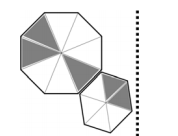
\includegraphics[width=0.3\columnwidth]{q5.png}
	\caption*{}
	\label{fig:q5}
\end{figure}

\hfill{\brak{\text{GATE XE 2022}}}
\begin{enumerate}
	\begin{multicols}{2}
	\item 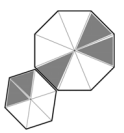
\includegraphics[width=0.8\linewidth]{q5a.png}
	\item 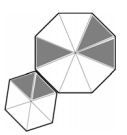
\includegraphics[width=0.8\linewidth]{q5b.png}
	\item 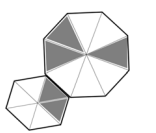
\includegraphics[width=0.8\linewidth]{q5c.png}
	\item 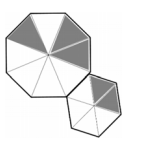
\includegraphics[width=0.8\linewidth]{q5d.png}
	\end{multicols}
\end{enumerate}

\item In the last few years, several new shopping malls were opened in the city. The total number of visitors in the malls is impressive. However, the total revenue generated through sales in the shops in these malls is generally low.
Which one of the following is the CORRECT logical inference based on the information in the above passage?

\hfill{\brak{\text{GATE XE 2022}}}
\begin{enumerate}
	\item Fewer people are visiting the malls but spending more
	\item More people are visiting the malls but not spending enough
	\item More people are visiting the malls and spending more
	\item Fewer people are visiting the malls and not spending enough
\end{enumerate}

\item In a partnership business the monthly investment by three friends for the first six months is in the ratio $3 \colon 4 \colon 5$. After six months, they had to increase their monthly investments by $10\%$, $15\%$ and $20\%$, respectively, of their initial monthly investment. The new investment ratio was kept constant for the next six months.
What is the ratio of their shares in the total profit \brak{\text{in the same order}} at the end of the year such that the share is proportional to their individual total investment over the year?

\hfill{\brak{\text{GATE XE 2022}}}
\begin{enumerate}
	\item $22 \colon 23 \colon 24$
	\item $22 \colon 33 \colon 50$
	\item $33 \colon 46 \colon 60$
	\item $63 \colon 86 \colon 110$
\end{enumerate}

\item Consider the following equations of straight lines:
\begin{align*}
	\text{Line L1} &\colon 2x - 3y = 5 \\
	\text{Line L2} &\colon 3x + 2y = 8 \\
	\text{Line L3} &\colon 4x - 6y = 5 \\
	\text{Line L4} &\colon 6x - 9y = 6
\end{align*}
Which one among the following is the correct statement?

\hfill{\brak{\text{GATE XE 2022}}}
\begin{enumerate}
	\item L1 is parallel to L2 and L1 is perpendicular to L3
	\item L2 is parallel to L4 and L2 is perpendicular to L1
	\item L3 is perpendicular to L4 and L3 is parallel to L2
	\item L4 is perpendicular to L2 and L4 is parallel to L3
\end{enumerate}

\item Given below are two statements and four conclusions drawn based on the statements.
\begin{description}
	\item[Statement 1:] Some soaps are clean.
	\item[Statement 2:] All clean objects are wet.
\end{description}
\begin{description}
	\item[Conclusion I:] Some clean objects are soaps.
	\item[Conclusion II:] No clean object is a soap.
	\item[Conclusion III:] Some wet objects are soaps.
	\item[Conclusion IV:] All wet objects are soaps.
\end{description}
Which one of the following options can be logically inferred?

\hfill{\brak{\text{GATE XE 2022}}}
\begin{enumerate}
	\item Only conclusion I is correct
	\item Either conclusion I or conclusion II is correct
	\item Either conclusion III or conclusion IV is correct
	\item Only conclusion I and conclusion III are correct
\end{enumerate}

\item An ant walks in a straight line on a plane leaving behind a trace of its movement. The initial position of the ant is at point P facing east.
The ant first turns $72\degree$ anticlockwise at P, and then does the following two steps in sequence exactly FIVE times before halting.
\begin{enumerate}
	\item moves forward for $10$ cm.
	\item turns $144\degree$ clockwise.
\end{enumerate}
The pattern made by the trace left behind by the ant is
\begin{figure}[H]
	\centering
	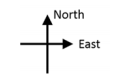
\includegraphics[width=0.2\columnwidth]{q10.png}
	\caption*{}
	\label{fig:q10}
\end{figure}

\hfill{\brak{\text{GATE XE 2022}}}
\begin{enumerate}
	\item 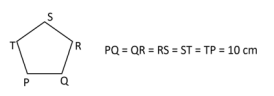
\includegraphics[width=0.5\columnwidth]{q10A.png}
        \item 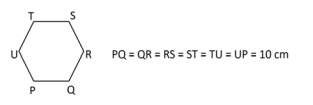
\includegraphics[width=0.5\columnwidth]{q10B.png}
	\item 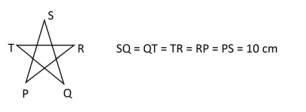
\includegraphics[width=0.5\columnwidth]{q10C.png}
	\item 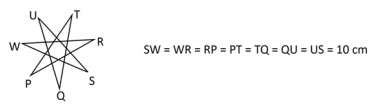
\includegraphics[width=0.5\columnwidth]{q10D.png}
\end{enumerate}

\item The value of $\lim_{x\to 0} \frac{1}{x} \int_{2}^{2+x} \brak{t + \sqrt{t^2+5}} dt$ is

\hfill{\brak{\text{GATE XE 2022}}}
\begin{enumerate}
	\begin{multicols}{4}
    \item $0$
    \item $4$
    \item $5$
    \item $6$
    \end{multicols}
\end{enumerate}

\item Let $\mathbb{C} = \{z = x+iy \colon x \text{ and } y \text{ are real numbers, } i = \sqrt{-1}\}$ be the set of complex numbers. Let the function $f(z) = u(x,y) + iv(x,y)$ for $z=x+iy \in \mathbb{C}$ be analytic in $\mathbb{C}$, where
$u(x,y) = xy^3 - yx^3$ and $v(x,y) = \frac{x^4}{4} + \frac{y^4}{4} - \frac{3}{2}x^2y^2$.
If $f'(z)$ denotes the derivative of $f(z)$, then

\hfill{\brak{\text{GATE XE 2022}}}
\begin{enumerate}
    \item $\abs{f'(-1+i)}^2 = 1$
    \item $\abs{f'(-1+i)}^2 = 7$
    \item $\abs{f'(-1+i)}^2 = 8$
    \item $\abs{f'(-1+i)}^2 = 10$
\end{enumerate}

\item If the partial differential equation
$(x+2)\frac{\partial^2 u}{\partial x^2} + 2(x+y)\frac{\partial^2 u}{\partial x \partial y} + 2(y-1)\frac{\partial^2 u}{\partial y^2} - 3y^2\frac{\partial u}{\partial y} = 0$
is parabolic on the circle $(x-a)^2 + (y-b)^2 = r^2$, then the values of $a, b$ and $r$ are given by

\hfill{\brak{\text{GATE XE 2022}}}
\begin{enumerate}
    \item $a=1, b=2, r=1$
    \item $a=-1, b=2, r=1$
    \item $a=1, b=-2, r=1$
    \item $a=-1, b=-2, r=1$
\end{enumerate}

\item Let $\Gamma$ be the positively oriented circle $x^2 + y^2 = 9$ in the $xy$-plane. If
$\oint_{\Gamma} (3y + e^{x \sin x}) dx + (7x + \sqrt{y^2+2}) dy = a\pi$,
where $a$ is a real constant, then $a$ is equal to \underline{\hspace{2cm}}.

\hfill{\brak{\text{GATE XE 2022}}}

\item Let $y_1(x)$ and $y_2(x)$ be two linearly independent solutions of
$x^2 \frac{d^2 y}{dx^2} - 2x \frac{dy}{dx} + 2y = 0, \quad x>0$.
Let $W(y_1, y_2)(x)$ denote the Wronskian of $y_1(x)$ and $y_2(x)$ at $x$.
If $W(y_1, y_2)(1) = 1$ then $W(y_1, y_2)(2)$ is equal to \underline{\hspace{2cm}}.

\hfill{\brak{\text{GATE XE 2022}}}

\item Let $A = \myvec{2 & 0 & 1 & 1 \\ 1 & 2 & 5 & -5 \\ 0 & 0 & 3 & 0 \\ 0 & 0 & 1 & 3}$. Then the sum of the geometric multiplicities of the distinct eigenvalues of $A$ is equal to \underline{\hspace{2cm}}.

\hfill{\brak{\text{GATE XE 2022}}}

\item In a cosmopolitan city, the population comprises of $30\%$ female and $70\%$ male. Suppose that $5\%$ of female and $30\%$ of male in the population are foreigners. A person is selected at random from this population. Given that the selected person is a foreigner, the probability that the person is a female is \underline{\hspace{2cm}} \brak{\text{round off to three decimal places}}.

\hfill{\brak{\text{GATE XE 2022}}}

\item Let $f \colon (0, \infty) \to \mathbb{R}$ be the continuous function such that $f(x) = 2 + \frac{g(x)}{x}$ for all $x>0$, where $g(x) = \int_{1}^{x} f(t) dt$ for all $x>0$. Then $f(2)$ is equal to

\hfill{\brak{\text{GATE XE 2022}}}
\begin{enumerate}
    \begin{multicols}{2}
    \item $2 + \log_e 2$
    \item $2 - \log_e 2$
    \item $2 + \log_e 4$
    \item $2 - \log_e 4$
    \end{multicols}
\end{enumerate}

\item Let $A$ and $B$ be $n \times n$ matrices with real entries.
Consider the following statements:
\begin{description}
    \item[P:] If $A$ is symmetric then $\text{rank}(A) = \text{Number of nonzero eigenvalues (counting multiplicity) of } A$.
    \item[Q:] If $AB = 0$ then $\text{rank}(A) + \text{rank}(B) \leq n$.
\end{description}
Then

\hfill{\brak{\text{GATE XE 2022}}}
\begin{enumerate}
    \item both P and Q are TRUE
    \item P is TRUE and Q is FALSE
    \item P is FALSE and Q is TRUE
    \item both P and Q are FALSE
\end{enumerate}

\item Let $f \colon \mathbb{R}^2 \to \mathbb{R}$ be given by $f(x,y) = 4xy - 2x^2 - y^4 + 1$. The number of critical points where $f$ has local maximum is equal to \underline{\hspace{2cm}}.

\hfill{\brak{\text{GATE XE 2022}}}

\item If the quadrature rule
$\int_{-1}^{1} f(x)dx \approx \alpha f(a) + \gamma f(\beta)$,
where $\alpha, \beta$ and $\gamma$ are real constants, is exact for all polynomials of degree $\leq 3$, then $\gamma + 3(\alpha^2 + \beta^2) + (\alpha^3 + \beta^3)$ is equal to \underline{\hspace{2cm}}.

\hfill{\brak{\text{GATE XE 2022}}}

\item A heavy horizontal cylinder of diameter D supports a mass of liquid having density $\rho$ as shown in the figure. Find out the vertical component of force exerted by the liquid per unit length of the cylinder if g is the acceleration due to gravity.
\begin{figure}[H]
    \centering
    
\includegraphics[width=0.4\columnwidth]{q22.png}
    \caption*{}
    \label{fig:q22}
\end{figure}

\hfill{\brak{\text{GATE XE 2022}}}
\begin{enumerate}
    \begin{multicols}{2}
    \item $\frac{\pi D^2}{4}\rho g$
    \item $\frac{\pi D^2}{8}\rho g$
    \item $\frac{\pi D^2}{2}\rho g$
    \item $\frac{\pi D^2}{3}\rho g$
    \end{multicols}
\end{enumerate}

\item The figure shows the developing zone and the fully developed region in a pipe flow where the steady flow takes place from left to right. The wall shear stress in the sections A, B, C, and D are given by $\tau_A, \tau_B, \tau_C$, and $\tau_D$, respectively. Select the correct statement.
\begin{figure}[H]
    \centering
    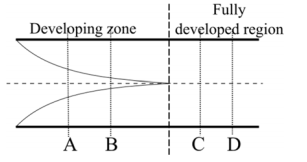
\includegraphics[width=0.6\columnwidth]{q23.png}
    \caption*{}
    \label{fig:q23}
\end{figure}

\hfill{\brak{\text{GATE XE 2022}}}
\begin{enumerate}
    \item $\tau_A > \tau_B$
    \item $\tau_B > \tau_A$
    \item $\tau_C > \tau_B$
    \item $\tau_C > \tau_D$
\end{enumerate}

\item The left hand column lists some non-dimensional numbers and the right hand column lists some physical phenomena. Indicate the correct combination
\begin{table}[h]
    \centering
    \begin{tabular}{|l|l|}
    \hline
    1. Reynolds number & i. Wave drag \\
    2. Froude number & ii. Compressible flow \\
    3. Mach number & iii. Viscous drag \\
    4. Weber number & iv. Spray formation \\
    \hline
    \end{tabular}
    \caption*{}
    \label{tab:q24}
\end{table}

\hfill{\brak{\text{GATE XE 2022}}}
\begin{enumerate}
    \item 1-iii, 2-i, 3-ii, 4-iv
    \item 1-i, 2-ii, 3-iv, 4-iii
    \item 1-iv, 2-iii, 3-iv, 4-iii
    \item 2-iv, 1-iii, 3-ii, 4-i
\end{enumerate}

\item As temperature increases

\hfill{\brak{\text{GATE XE 2022}}}
\begin{enumerate}
    \item the dynamic viscosity of a gas increases.
    \item the dynamic viscosity of a liquid decreases.
    \item the dynamic viscosity of a liquid does not change.
    \item the dynamic viscosity of a gas decreases.
\end{enumerate}

\item Which of the following statement(s) regarding a venturimeter is/are correct?

\hfill{\brak{\text{GATE XE 2022}}}
\begin{enumerate}
    \item In the direction of flow, it consists of a converging section, a throat, and a diverging section.
    \item In the direction of flow, it consists of a diverging section, a throat, and a converging section.
    \item It is used for flow measurement at a very low Reynolds number.
    \item Pressure tappings are provided just upstream of the venturimeter and at the throat.
\end{enumerate}

\item Which of the following statement(s) is/are true for streamlines in a steady incompressible flow?

\hfill{\brak{\text{GATE XE 2022}}}
\begin{enumerate}
    \item Two streamlines cannot intersect each other.
    \item Flow rate increases between two diverging streamlines.
    \item Flow rate decreases between two diverging streamlines.
    \item Stream function has a constant value along a streamline.
\end{enumerate}

\item A flow has a velocity potential given by $\phi = Ax^3$ where 'A' is a non-zero constant. Which of the following statement(s) is/are true about the flow?

\hfill{\brak{\text{GATE XE 2022}}}
\begin{enumerate}
    \item The flow is incompressible.
    \item The flow is irrotational.
    \item The flow has local acceleration.
    \item The flow has convective acceleration.
\end{enumerate}

\item A boundary layer develops due to a two-dimensional steady flow over a horizontal flat plate. Consider a vertical line away from the leading edge which extends from the wall to the edge of the boundary layer. Which of the following quantity/quantities is/are not constant along the vertical line? $u$ and $v$ represent the components of velocity in the direction along the plate and normal to it, respectively and x is taken along the length of the plate while p is the pressure. Neglect body forces.

\hfill{\brak{\text{GATE XE 2022}}}
\begin{enumerate}
    \begin{multicols}{2}
    \item $u$
    \item $\frac{\partial u}{\partial x}$
    \item $v$
    \item $p$
    \end{multicols}
\end{enumerate}

\item A 10 kg mass placed on an infinitely long horizontal massless flat platform is to be supported by a steady vertical water jet as shown in the figure. The diameter of the jet is 5 cm. What minimum average velocity is required to hold the mass in place? Assume $\rho_{water} = 1000 \text{ kg/m}^3, g = 10 \frac{\text{m}}{\text{s}^2}$ and $\pi = 3.14$. Neglect friction. (Round off to two decimal places)
\begin{figure}[H]
    \centering
    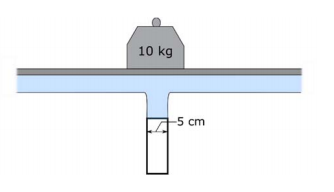
\includegraphics[width=0.5\columnwidth]{q30.png}
    \caption*{}
    \label{fig:q30}
\end{figure}

\hfill{\brak{\text{GATE XE 2022}}}

\item Consider an inviscid flow through a smooth pipe which has a pitot-static tube arrangement as shown. Find the centre-line velocity in the pipe. Consider that the density of the fluid is 1000 kg/m$^3$, acceleration due to gravity is 10 m/s$^2$, and the specific gravity of the manometric fluid is 11.
\begin{figure}[H]
    \centering
    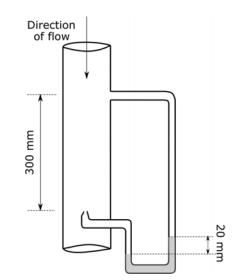
\includegraphics[width=0.3\columnwidth]{q31.png}
    \caption*{}
    \label{fig:q31}
\end{figure}

\hfill{\brak{\text{GATE XE 2022}}}
\begin{enumerate}
    \begin{multicols}{2}
    \item 2 m/s
    \item 3 m/s
    \item 5 m/s
    \item 7 m/s
    \end{multicols}
\end{enumerate}

\item The speed of propagation, c, of a capillary wave depends on the density of the fluid, $\rho$, the wavelength of the wave, $\lambda$, and the surface tension, $\sigma$. If the density and wavelength remain constant, halving the surface tension would lead to a new velocity, c', given by

\hfill{\brak{\text{GATE XE 2022}}}
\begin{enumerate}
    \item $c' = 2c$
    \item $c' = \sqrt{2}c$
    \item $c' = \frac{c}{\sqrt{2}}$
    \item $c' = c$
\end{enumerate}

\item A two-dimensional flow field is described by a combination of a source of strength m at the origin and a uniform flow, U, in the positive x-direction such that the velocity potential is given by
$\phi = Ux + \frac{m}{2\pi} \ln{\sqrt{x^2+y^2}}$
The stagnation streamline is shown in the figure. Find the distance aa'.
\begin{figure}[H]
    \centering
    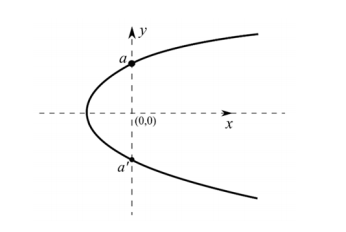
\includegraphics[width=0.4\columnwidth]{q33.png}
    \caption*{}
    \label{fig:q33}
\end{figure}

\hfill{\brak{\text{GATE XE 2022}}}
\begin{enumerate}
    \begin{multicols}{2}
    \item $\frac{m}{U}$
    \item $\frac{2m}{U}$
    \item $\frac{8m}{U}$
    \item $\frac{m}{2U}$
    \end{multicols}
\end{enumerate}

\item A typical boundary layer over a flat plate has a linear velocity profile with zero velocity at the wall and freestream velocity, U$_\infty$, at the outer edge of the boundary layer. What is the ratio of the momentum thickness to the thickness of the boundary layer?

\hfill{\brak{\text{GATE XE 2022}}}
\begin{enumerate}
    \begin{multicols}{4}
    \item $\frac{1}{2}$
    \item $\frac{1}{4}$
    \item $\frac{1}{6}$
    \item $\frac{1}{3}$
    \end{multicols}
\end{enumerate}

\item Identify the configuration(s) in which steady two-dimensional internal flow may show boundary layer separation if the flow direction is left to right.

\hfill{\brak{\text{GATE XE 2022}}}
\begin{enumerate}
    \begin{multicols}{2}
    \item 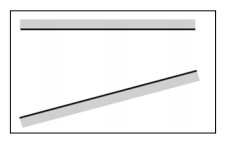
\includegraphics[width=0.9\linewidth]{q35A.png}
    \item 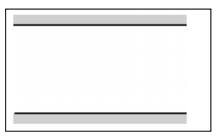
\includegraphics[width=0.9\linewidth]{q35B.png}
    \item 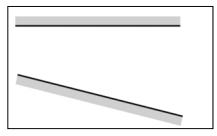
\includegraphics[width=0.9\linewidth]{q35C.png}
    \item 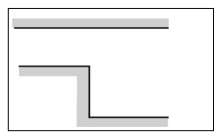
\includegraphics[width=0.9\linewidth]{q35D.png}
    \end{multicols}
\end{enumerate}

\item Consider steady fully developed flow of a liquid through two large horizontal flat parallel plates separated by a distance of 2 mm. One of the plate is fixed and the other plate moves at a speed of 0.5 m/s. What is the magnitude of the pressure gradient (in Pa/m) in the direction of the flow required to ensure that the net flow through the plates is zero?
Dynamic viscosity of the liquid is 5x10$^{-4}$ Ns/m$^2$
(Round off to the nearest integer)

\hfill{\brak{\text{GATE XE 2022}}}

\item Consider two-dimensional turbulent flow of air over a horizontal flat plate of length 1 m. Skin friction coefficient at a length x from the leading edge of the plate is obtained as:
$c_f = \frac{0.06}{(\text{Re}_x)^{0.2}}$
where, Re$_x$ is the local Reynolds number.
Find out the drag force per unit width (in N/m$^2$) on the plate if the free stream air velocity is 10 m/s.
Density and dynamic viscosity of air are given as 1.2 kg/m$^3$ and 1.83x10$^{-5}$ N-s/m$^2$, respectively.
(Round off to three decimal places)

\hfill{\brak{\text{GATE XE 2022}}}

\item For an inviscid fluid with density 1 kg/m$^3$, the Cartesian velocity field is given as:
$\mathbf{u} = (-2x+y)t\mathbf{i} + (2x+y)t\mathbf{j}$ m/s
Neglecting the body forces, find the magnitude of pressure gradient in (Pa/m) at (x, y) = (1 m, 1 m) at t = 1 s.
(Round off to two decimal places)

\hfill{\brak{\text{GATE XE 2022}}}

\item Consider a lawn sprinkler with horizontal arms of radius, a = 10 cm which has water introduced vertically through the centre, as shown in the figure. The exit area of the jet is 25 cm$^2$ and the jet velocity is 1 m/s. The water is ejected orthogonal to the sprinkler arm and the jet makes an angle of 60$\degree$ with the horizontal plane. Find the torque (in N-m) required to hold the sprinkler stationary. Consider water density 1000 kg/m$^3$. Neglect the effects of friction and gravity.
(Round off to two decimal places)
\begin{figure}[H]
    \centering
    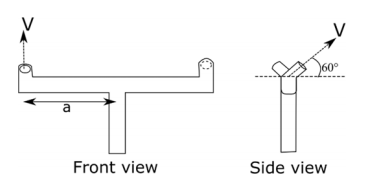
\includegraphics[width=0.6\columnwidth]{q39.png}
    \caption*{}
    \label{fig:q39}
\end{figure}

\hfill{\brak{\text{GATE XE 2022}}}

\item A wooden cylinder (specific gravity = 0.6) of length L and diameter D floats in water (density 1000 kg/m$^3$). Find out the minimum value of D/L for which the cylinder floats with its axis vertical.
(Round off to three decimal places)

\hfill{\brak{\text{GATE XE 2022}}}

\item Consider a cart of mass 10 kg placed on an inclined plane (angle of inclination 60$\degree$ with horizontal) as shown in the figure. A turning vane of negligible weight is mounted on the cart. A horizontal steady water jet is issued from a stationary nozzle of area 0.1 m$^2$ and strikes the turning vane as shown in the figure. The vane turns the jet downward parallel to the inclined plane. Find out the minimum jet velocity (in m/s) which will not allow the cart to come down. Neglect friction, consider density of water = 1000 kg/m$^3$ and acceleration due to gravity = 10 m/s$^2$.
(Round off to two decimal places)
\begin{figure}[H]
    \centering
    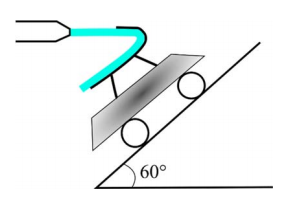
\includegraphics[width=0.6\columnwidth]{q41.png}
    \caption*{}
    \label{fig:q41}
\end{figure}

\hfill{\brak{\text{GATE XE 2022}}}

\item A siphon is used to drain out water (density 1000 kg/m$^3$) from a tank as shown in the figure. What can be the maximum height z (in meter) of the point C? Consider acceleration due to gravity = 10 m/s$^2$, pressure at point A = 101 kPa, vapour pressure of water = 29.5 kPa and neglect friction.
(Round off to two decimal places)
\begin{figure}[H]
    \centering
    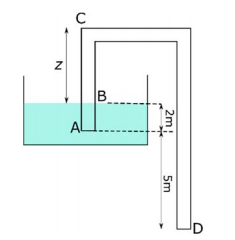
\includegraphics[width=0.3\columnwidth]{q42.png}
    \caption*{}
    \label{fig:q42}
\end{figure}

\hfill{\brak{\text{GATE XE 2022}}}

\item The horizontal belt of negligible weight shown in the figure moves with a steady velocity (V) of 2.5 m/s and skims over the top surface of an oil-film of depth h = 3 cm. The length (L) and width (b) of the belt are, respectively, 2 m and 60 cm. Find the viscosity of the oil (in Pa-s), given that the minimum power required to move the belt is 100 W. Neglect the end effects.
(Round off to two decimal places)
\begin{figure}[H]
    \centering
    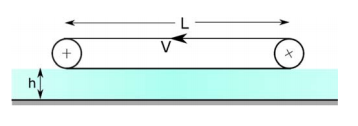
\includegraphics[width=0.5\columnwidth]{q43.png}
    \caption*{}
    \label{fig:q43}
\end{figure}

\hfill{\brak{\text{GATE XE 2022}}}

\item Number of atoms per unit area of the \brak{110} plane of a body centered cubic crystal, with lattice parameter 'a', is

\hfill{\brak{\text{GATE XE 2022}}}
\begin{enumerate}
    \begin{multicols}{2}
    \item $\frac{1}{a^2}$
    \item $\frac{\sqrt{2}}{a^2}$
    \item $\frac{1}{\sqrt{3}a^2}$
    \item $\frac{1}{\sqrt{2}a^2}$
    \end{multicols}
\end{enumerate}

\item Match the following materials with their corresponding bonding types.
\begin{table}[h]
    \centering
    \begin{tabular}{|l|l|}
    \hline
    \textbf{Material} & \textbf{Bonding} \\
    \hline
    P: Cu$_{0.5}$Al$_{0.5}$ & 1: Ionic \\
    Q: ZnS & 2: Covalent \\
    R: Na$_2$O & 3: Metallic \\
    S: Li$_4$SiO$_4$ & 4: Mixed \\
    \hline
    \end{tabular}
    \caption*{}
    \label{tab:q45}
\end{table}

\hfill{\brak{\text{GATE XE 2022}}}
\begin{enumerate}
    \item P - 4; Q - 2; R - 3; S - 1
    \item P - 3; Q - 4; R - 2; S - 1
    \item P - 3; Q - 2; R - 1; S - 4
    \item P - 3; Q - 1; R - 4; S - 2
\end{enumerate}

\item In an ideal rubber, the primary factor responsible for elasticity up to small strains is

\hfill{\brak{\text{GATE XE 2022}}}
\begin{enumerate}
    \item Change in both enthalpy and entropy
    \item Change in enthalpy, but no change in the entropy
    \item No change in enthalpy, but change in the entropy
    \item Neither a change in enthalpy, nor a change in the entropy
\end{enumerate}

\item Which one of the following statements is true for an intrinsic semiconductor?

\hfill{\brak{\text{GATE XE 2022}}}
\begin{enumerate}
    \item Electrical conductivity increases with increasing temperature and pressure
    \item Electrical conductivity increases with increasing temperature and decreasing pressure
    \item Electrical conductivity increases with decreasing temperature and increasing pressure
    \item Electrical conductivity increases with decreasing temperature and pressure
\end{enumerate}

\item A differential scanning calorimetry (DSC) experiment tracks the heat flow into or out of a system as a function of temperature. If the experiments given in the options below are performed at 1 atmospheric pressure, then in which case will the DSC thermogram exhibit a spike, either upward or downward?

\hfill{\brak{\text{GATE XE 2022}}}
\begin{enumerate}
    \item Heating 10 mg of pure Cu from 323 K to 673 K
    \item Cooling pure water from 323 K to 278 K
    \item Heating pure ice from 263 K to 284 K
    \item Cooling a Pb-Sn alloy at the eutectic composition from 323 K to 273 K
\end{enumerate}

\item Which one of the following solvent environments will likely result in swelling of solid polystyrene?

\hfill{\brak{\text{GATE XE 2022}}}
\begin{enumerate}
    \item 0.1 M NaOH in H$_2$O
    \item HCl (aq.) of pH = 6
    \item Distilled water
    \item Benzene
\end{enumerate}

\item Vickers microhardness (HV) of a ductile material A is higher than another ductile material B. Which of the following is/are true?

\hfill{\brak{\text{GATE XE 2022}}}
\begin{enumerate}
    \item Young's modulus of A is greater than B
    \item Yield strength of A is greater than B
    \item Scratch resistance of A is greater than B
    \item Ductility of A is greater than B
\end{enumerate}

\item The enthalpy required to create an oxygen vacancy in CeO$_2$ is 4 eV. The number of oxygen vacancies present per mole of CeO$_2$ at 1000 K is \underline{\hspace{2cm}}.
(Round off to the nearest integer)
Given:
$N_A$: Avogadro's number = $6.02 \times 10^{23}$ mole$^{-1}$
$k_B$: Boltzmann's constant = $8.62 \times 10^{-5}$ eV/K

\hfill{\brak{\text{GATE XE 2022}}}

\item An electrochemical reaction is known to occur at +4.50 V against a Li$^+$/Li reference electrode. The potential of the same reaction against a Zn$^{2+}$/Zn reference electrode is \underline{\hspace{2cm}} V. (Round off to two decimal places).
Given:
E$^0$ (Li$^+$/Li) = -3.04 V versus Standard Hydrogen Electrode
E$^0$ (Zn$^{2+}$/Zn) = -0.77 V versus Standard Hydrogen Electrode

\hfill{\brak{\text{GATE XE 2022}}}

\item For a binary system at constant pressure, there are two types of invariant reactions:
(i) $\alpha \leftrightarrow \beta + \gamma$
(ii) $\alpha + \beta \leftrightarrow \gamma$
Analogously, how many different types of invariant reactions may exist under variable temperature and pressure, for a binary system?

\hfill{\brak{\text{GATE XE 2022}}}
\begin{enumerate}
    \begin{multicols}{4}
    \item 1
    \item 2
    \item 3
    \item 4
    \end{multicols}
\end{enumerate}

\item For a glass marginally below its glass transition temperature, which one of the following statements is true?

\hfill{\brak{\text{GATE XE 2022}}}
\begin{enumerate}
    \item Glass has higher enthalpy than both the corresponding crystalline and liquid phases
    \item Glass has lower enthalpy than both the corresponding crystalline and liquid phases
    \item Glass has higher entropy than the corresponding crystalline phase and lower entropy than the corresponding liquid phase
    \item Glass has lower entropy than the corresponding crystalline phase and higher entropy than the corresponding liquid phase
\end{enumerate}

\item Which one of the following samples of high-purity aluminium (Al) single crystal will plastically yield at the lowest applied load under ambient conditions? Loading axis is along the direction shown in the schematic.
\begin{figure}[H]
    \centering
    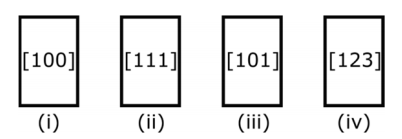
\includegraphics[width=0.7\columnwidth]{q55.png}
    \caption*{}
    \label{fig:q55}
\end{figure}

\hfill{\brak{\text{GATE XE 2022}}}
\begin{enumerate}
    \item (i)
    \item (ii)
    \item (iii)
    \item (iv)
\end{enumerate}

\item Refer to the schematic shown. Two dog-bone samples, labelled 1 and 2, of a Cu alloy are tested under tension at room temperature to points "E" and "P", respectively. Subsequently, they are unloaded completely and metallographically polished. Brinell hardness testing was performed in the gauge section of the samples. Which one of the following can be inferred about the measured Brinell hardness number (BHN)?
\begin{figure}[H]
    \centering
    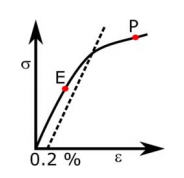
\includegraphics[width=0.4\columnwidth]{q56.png}
    \caption*{}
    \label{fig:q56}
\end{figure}

\hfill{\brak{\text{GATE XE 2022}}}
\begin{enumerate}
    \item BHN of 1 $>$ BHN of 2
    \item BHN of 1 = BHN of 2
    \item BHN of 1 $<$ BHN of 2
    \item A conclusion about BHN of samples 1 and 2 cannot be made, with the provided information
\end{enumerate}

\item During the ageing of a homogenized Al-Cu alloy (1 to 4 wt.\% Cu) below the GP zone solvus, hardness of the alloy:

\hfill{\brak{\text{GATE XE 2022}}}
\begin{enumerate}
    \item increases monotonically
    \item decreases monotonically
    \item first increases and then decreases
    \item first decreases and then increases
\end{enumerate}

\item A student aims to deposit a thin metallic film on SiO$_2$ substrate, with an adhesion layer between the metal film and substrate, in a contiguous planar fashion. Island type of growth must be avoided. The student performs an extensive optimization exercise. Which one of the following steps is in the right direction?

\hfill{\brak{\text{GATE XE 2022}}}
\begin{enumerate}
    \item Choose a metallic adhesion layer with very low interfacial energy with the deposited thin film
    \item Choose a metallic adhesion layer with very low interfacial energy with SiO$_2$, irrespective of its interaction with metal film to be deposited
    \item Increase the substrate temperature and decrease the deposition rate
    \item Use intermittent stages of deposition followed by annealing
\end{enumerate}

\item For a diffusional transformation (i.e., growth of $\beta$ precipitates in an $\alpha$ matrix), which of the following is/are true with increasing degree of undercooling?

\hfill{\brak{\text{GATE XE 2022}}}
\begin{enumerate}
    \item Rate of transformation first increases and then decreases
    \item Rate of transformation first decreases and then increases
    \item Thermodynamic driving force increases monotonically
    \item Mobility of atoms in $\alpha$ matrix remains unchanged
\end{enumerate}

\item A two-phase ($\alpha + \beta$) mixture of an A-B binary system has the following properties:
(i) Phase $\alpha$ has equal weight percentages of A and B.
(ii) Phase $\beta$ has twice the mole fraction of A compared to B.
(iii) The two-phase mixture has equal amounts of $\alpha$ and $\beta$.
(iv) Atomic mass of A is twice that of B.
The mole fraction of A in the resultant two-phase mixture is \underline{\hspace{2cm}}.
(Round off to one decimal)

\hfill{\brak{\text{GATE XE 2022}}}

\item It is known that component A diffuses into a solid to a depth of 10 $\mu$m in 1 hour at 300 K. Treat diffusion in one dimension. The time taken for A to diffuse to the same depth at 600 K is \underline{\hspace{2cm}} seconds. (Round off to 1 decimal).
Diffusivity of A in the solid is given by
$D_A = D_A^0 \exp\brak{-\frac{E_a}{k_B T}}$
$D_A^0$: Diffusivity coefficient
$E_a$: Activation energy = 0.3 eV
$k_B$: Boltzmann's constant = $8.62 \times 10^{-5}$ eV/K
$T$: Absolute temperature

\hfill{\brak{\text{GATE XE 2022}}}

\item A spherical $\beta$ particle nucleates from the $\alpha$ matrix on a non-deformable substrate $\delta$, forming a contact angle of $\theta$ as shown in the schematic.
The value of $\frac{\Delta G_{het}^*}{\Delta G_{hom}^*}$ is \underline{\hspace{2cm}}. (Round off to three decimal places)
\begin{figure}[H]
    \centering
    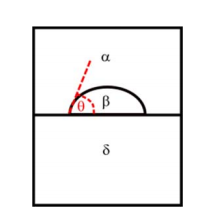
\includegraphics[width=0.3\columnwidth]{q62.png}
    \caption*{}
    \label{fig:q62}
\end{figure}
$\Delta G_{hom}^*$ = Gibbs free energy change at the critical radius for homogeneous nucleation
$\Delta G_{het}^*$ = Gibbs free energy change at the critical radius for heterogeneous nucleation
$\alpha$-$\beta$ interfacial energy = 0.4 J/m$^2$
$\alpha$-$\delta$ interfacial energy = 0.3 J/m$^2$
$\beta$-$\delta$ interfacial energy = 0.02 J/m$^2$

\hfill{\brak{\text{GATE XE 2022}}}

\item The resistivity of a pure semiconductor at 298 K is 3000 $\ohm$m. Assume that the number of electrons excited ($n_e$) across the band gap is given by the relation
$n_e = N_A \exp\brak{-\frac{E_g}{k_B T}}$
$N_A$: Avogadro's number = $6.02 \times 10^{23}$ mole$^{-1}$
$k_B$: Boltzmann's constant = $8.62 \times 10^{-5}$ eV/K
$T$: Absolute temperature
Mobility of electrons in the semiconductor = 0.14 m$^2$/(V s)
Mobility of holes in the semiconductor = 0.06 m$^2$/(V s)
Absolute charge of an electron = $1.60 \times 10^{-19}$ C
The band gap ($E_g$) of the semiconductor is \underline{\hspace{2cm}} eV.
(Round off to two decimals)

\hfill{\brak{\text{GATE XE 2022}}}

\item A new glass material is developed to minimize the transmission of the light through the window with glass panel of thickness 5 mm. The refractive index of the glass material is 1.5 and the absorption coefficient can be changed from 0.3 cm$^{-1}$ to 1 cm$^{-1}$. In the given range of absorption coefficients, the ratio of the maximum to the minimum fraction of the light coming out of the other side of the glass panel is \underline{\hspace{2cm}}. (Round off to two decimal places)

\hfill{\brak{\text{GATE XE 2022}}}

\item The third peak in the X-ray diffraction pattern of a face-centered cubic crystal is at 2$\theta$ value of 45$\degree$, where 2$\theta$ is the angle between the incident and reflected rays. The wavelength of the monochromatic X-ray beam is 1.54 \AA. Considering first-order reflection, the lattice parameter of the crystal is \underline{\hspace{2cm}} \AA. (Round off to two decimal places)

\hfill{\brak{\text{GATE XE 2022}}}

\item A force $F$ is applied at an angle $\theta = 30\degree$ on an elastic column as shown in the figure. $E$ and $I$ are respectively the Young's modulus and area moment of inertia. The smallest magnitude of $F$ needed to cause buckling is
\begin{figure}[H]
    \centering
    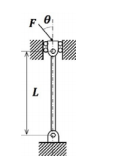
\includegraphics[width=0.2\columnwidth]{q66.png}
    \caption*{}
    \label{fig:q66}
\end{figure}

\hfill{\brak{\text{GATE XE 2022}}}
\begin{enumerate}
    \item $\frac{2}{\sqrt{3}}\frac{\pi^2 EI}{L^2}$
    \item $\frac{\sqrt{3}}{2}\frac{\pi^2 EI}{L^2}$
    \item $\frac{\pi^2 EI}{2L^2}$
    \item $\frac{2\pi^2 EI}{L^2}$
\end{enumerate}

\item The shear stress due to a transverse shear force in a linear elastic isotropic beam of rectangular cross-section

\hfill{\brak{\text{GATE XE 2022}}}
\begin{enumerate}
    \item varies linearly along the depth in the transverse direction of the beam
    \item is zero at the neutral axis
    \item is maximum at the neutral axis
    \item remains constant along the depth in the transverse direction of the beam
\end{enumerate}

\item A massless semicircular rod held fixed at end A is in the xy-plane, as shown in the figure. A force P along the negative z direction is acting at point B on the rod. The unit vectors along x, y and z directions are denoted respectively as i, j and k. Due to the applied force P, the cross-section of the rod at point D will be subjected to
\begin{figure}[H]
    \centering
    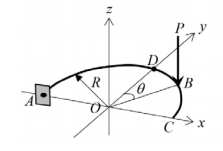
\includegraphics[width=0.4\columnwidth]{q68.png}
    \caption*{}
    \label{fig:q68}
\end{figure}

\hfill{\brak{\text{GATE XE 2022}}}
\begin{enumerate}
    \item a twisting moment $PR(1-\cos\theta)\mathbf{i}$, a bending moment $PR\sin\theta\mathbf{j}$, and a shear force $-P\mathbf{k}$
    \item a twisting moment $PR(1-\sin\theta)\mathbf{i}$, a bending moment $PR\cos\theta\mathbf{j}$, and a shear force $P\mathbf{k}$
    \item a twisting moment $PR(\cos\theta-1)\mathbf{i}$, a bending moment $-PR\sin\theta\mathbf{j}$, and a shear force $-P\mathbf{k}$
    \item a twisting moment $PR\sin\theta\mathbf{i}$, a bending moment $PR(1-\cos\theta)\mathbf{j}$, and a shear force $P\mathbf{k}$
\end{enumerate}

\item In the truss shown in the figure, all the members are pin jointed to each other. The members AB, BD, DE and DC have the same length. For the given loading, which of the following is the correct statement?
\begin{figure}[H]
    \centering
    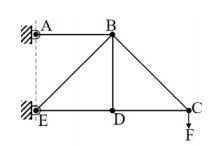
\includegraphics[width=0.5\columnwidth]{q69.png}
    \caption*{}
    \label{fig:q69}
\end{figure}

\hfill{\brak{\text{GATE XE 2022}}}
\begin{enumerate}
    \item BD is a zero-force member, and AB and ED are in compression
    \item AB is in tension, ED is in compression, and BD is a zero-force member
    \item AB and DC are in tension, and BC is in compression
    \item ED is in tension, and DC and BC are in compression
\end{enumerate}

\item End B of the 2 m long rigid rod AB is constrained to move horizontally in the slot as shown in the figure and has a velocity of 1.0 $\mathbf{i}$ m/s. The angular velocity of the rod at the instant shown is 2 rad/s. The unit vectors along x and y directions are denoted respectively as $\mathbf{i}$ and $\mathbf{j}$. The velocity of point A in m/s is then given by
\begin{figure}[H]
    \centering
    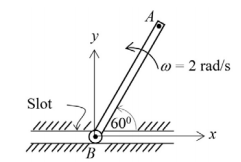
\includegraphics[width=0.4\columnwidth]{q70.png}
    \caption*{}
    \label{fig:q70}
\end{figure}

\hfill{\brak{\text{GATE XE 2022}}}
\begin{enumerate}
    \item $(1-2\sqrt{3})\mathbf{i} + 2\mathbf{j}$
    \item $(1+2\sqrt{3})\mathbf{i} - 2\mathbf{j}$
    \item $-2\sqrt{3}\mathbf{i} + 2\mathbf{j}$
    \item $2\sqrt{3}\mathbf{i} - 2\mathbf{j}$
\end{enumerate}

\item The assembly of four masses connected by rigid mass-less rods is kept on a smooth horizontal floor as shown in the figure. Under the applied force 2F, the magnitude of angular acceleration of the assembly at the instant shown is
\begin{figure}[H]
    \centering
    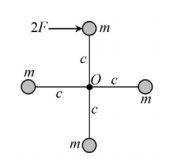
\includegraphics[width=0.3\columnwidth]{q71.png}
    \caption*{}
    \label{fig:q71}
\end{figure}

\hfill{\brak{\text{GATE XE 2022}}}
\begin{enumerate}
    \item $\frac{F}{mc}$
    \item $\frac{F}{2mc}$
    \item $\frac{2F}{3mc}$
    \item $\frac{F}{3mc}$
\end{enumerate}

\item A particle is constrained to move at a constant speed on an inclined plane (ABCD) along the curved path shown in the figure. Edges AD and BC are parallel to the y-axis. The inclined plane makes an angle $\theta$ with the $xy$-plane. The velocity vector of the particle makes an angle $\phi$ with the dotted line which is parallel to edge AB. If the speed of the particle is 2 m/s, $\phi=30\degree$, and $\theta=40\degree$, then the z-component of the velocity of the particle in m/s is \underline{\hspace{2cm}}
\begin{figure}[H]
    \centering
    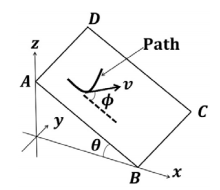
\includegraphics[width=0.4\columnwidth]{q72.png}
    \caption*{}
    \label{fig:q72}
\end{figure}

\hfill{\brak{\text{GATE XE 2022}}}
\begin{enumerate}
    \item $-1.32$
    \item $-1.00$
    \item $-1.11$
    \item $-1.50$
\end{enumerate}

\item A uniform elastic rod of constant cross-section is fixed at its left end as shown in the figure. An axial force $P$ is acting as shown. Assume that plane sections remain plane during deformation. The ratio of axial displacements at point A $(x=4L)$ to that at point B $(x=L)$ is \underline{\hspace{2cm}} (rounded off to one decimal place)
\begin{figure}[H]
    \centering
    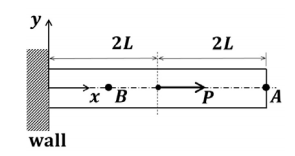
\includegraphics[width=0.5\columnwidth]{q73.png}
    \caption*{}
    \label{fig:q73}
\end{figure}

\hfill{\brak{\text{GATE XE 2022}}}

\item A thin-walled spherical pressure vessel has a mean radius of 500 mm and wall thickness of 10 mm. The yield strength of the material is 500 MPa. The internal pressure in MPa at which the spherical pressure vessel will yield according to the Tresca criterion is \underline{\hspace{2cm}} (rounded off to one decimal place)

\hfill{\brak{\text{GATE XE 2022}}}

\item The beam in the figure is subjected to a moment $M_0$ at mid span as shown. Which of the following is the vertical reaction at B?
\begin{figure}[H]
    \centering
    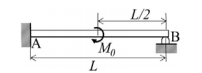
\includegraphics[width=0.5\columnwidth]{q75.png}
    \caption*{}
    \label{fig:q75}
\end{figure}

\hfill{\brak{\text{GATE XE 2022}}}
\begin{enumerate}
    \item $\frac{9M_0}{8L}$
    \item $\frac{15M_0}{8L}$
    \item $\frac{3M_0}{4L}$
    \item $\frac{9M_0}{4L}$
\end{enumerate}

\item A spring-mass system having a mass m and spring constant k, placed horizontally on a foundation, is connected to a vertically hanging mass m with the help of an inextensible string. Ignore the friction in the pulleys and also the inertia of pulleys, string and spring. Gravity is acting vertically downward as shown. The natural frequency of the system in rad/s is
\begin{figure}[H]
    \centering
    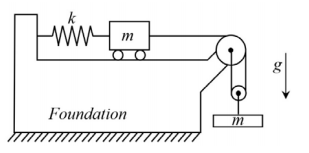
\includegraphics[width=0.6\columnwidth]{q76.png}
    \caption*{}
    \label{fig:q76}
\end{figure}

\hfill{\brak{\text{GATE XE 2022}}}
\begin{enumerate}
    \item $\sqrt{\frac{4k}{3m}}$
    \item $\sqrt{\frac{k}{2m}}$
    \item $\sqrt{\frac{k}{3m}}$
    \item $\sqrt{\frac{4k}{5m}}$
\end{enumerate}

\item One end of a uniform rigid rod OA of length L and mass m is attached to a frictionless hinge at O. The other end of the rod is connected to the roof at B with a mass-less inextensible thread AB. Initially the rod is horizontal and at rest. The gravity is acting vertically downward as shown. Immediately after the thread AB is cut, the reaction on the rod at O is
\begin{figure}[H]
    \centering
    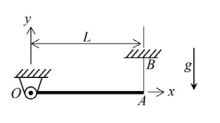
\includegraphics[width=0.5\columnwidth]{q77.png}
    \caption*{}
    \label{fig:q77}
\end{figure}

\hfill{\brak{\text{GATE XE 2022}}}
\begin{enumerate}
    \item $\frac{mg}{4}$ in the positive y-direction
    \item $\frac{mg}{2}$ in the negative y-direction
    \item $\frac{3mg}{4}$ in the negative y-direction
    \item $mg$ in the positive y-direction
\end{enumerate}

\item A circular shaft is rigidly connected to a wall at one end. The shaft has a solid portion and a hollow portion as shown in the figure. The length of each portion is $L$ and the shear modulus of the material is $G$. The polar moment of inertia of the hollow portion is $J$ and that of the solid portion is $50J$. A torque $T$ is applied at the right most end as shown. The rotation of the section PQ is
\begin{figure}[H]
    \centering
    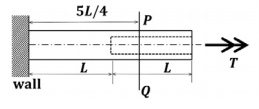
\includegraphics[width=0.5\columnwidth]{q78.png}
    \caption*{}
    \label{fig:q78}
\end{figure}

\hfill{\brak{\text{GATE XE 2022}}}
\begin{enumerate}
    \item $\frac{27TL}{100JG}$
    \item $\frac{TL}{40JG}$
    \item $\frac{5TL}{4JG}$
    \item $\frac{3TL}{4JG}$
\end{enumerate}

\item A rectangular plate of uniform thickness having initial length a and width b is placed between two rigid immovable walls. The temperature of the plate is increased by $\Delta T$. The plate is free to expand along the y and z directions. The mid-surface of the plate remains in the xy-plane. The Poisson's ratio is $\nu$ and the coefficient of thermal expansion is $\alpha$. Assuming that the plate is initially free of stresses, the change in length of the plate after the increase in temperature is given by
\begin{figure}[H]
    \centering
    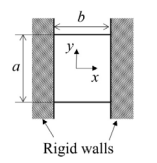
\includegraphics[width=0.4\columnwidth]{q79.png}
    \caption*{}
    \label{fig:q79}
\end{figure}

\hfill{\brak{\text{GATE XE 2022}}}
\begin{enumerate}
    \item $a(1-\nu)\alpha\Delta T$
    \item $a(1+\nu)\alpha\Delta T$
    \item $a\alpha\Delta T$
    \item $2a\alpha\Delta T$
\end{enumerate}

\item A mass m = 10 kg is attached to a spring as shown in the figure. The coefficient of friction between the mass and the inclined plane is 0.25. Assume that the acceleration due to gravity is 10 m/s$^2$ and that static and kinematic friction coefficients are the same. Equilibrium of the mass is impossible if the spring force is
\begin{figure}[H]
    \centering
    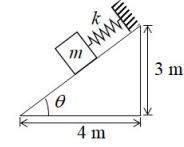
\includegraphics[width=0.4\columnwidth]{q80.png}
    \caption*{}
    \label{fig:q80}
\end{figure}

\hfill{\brak{\text{GATE XE 2022}}}
\begin{enumerate}
    \begin{multicols}{2}
    \item 30 N
    \item 45 N
    \item 60 N
    \item 75 N
    \end{multicols}
\end{enumerate}

\item The frame shown in the figure is subjected to a uniformly distributed load of 1000 N/m over a distance of 0.6 m. Neglecting the weight of the frame, the maximum shear force (in N) in the region between the supports A and B of the frame is \underline{\hspace{2cm}}.
\begin{figure}[H]
    \centering
    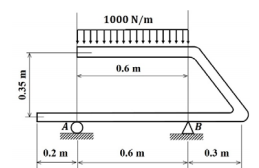
\includegraphics[width=0.6\columnwidth]{q81.png}
    \caption*{}
    \label{fig:q81}
\end{figure}

\hfill{\brak{\text{GATE XE 2022}}}

\item A slider moving in a frictionless slot is connected with a linear spring OA as shown in the figure. The following is known: stiffness of the spring = 2 kN/m, mass of the slider = 10 kg, and the unstretched length of the spring = 1 m. If the slider is released from rest at A the magnitude of its velocity (in m/s) when it passes through point B is \underline{\hspace{2cm}}(rounded off to the nearest integer)
\begin{figure}[H]
    \centering
    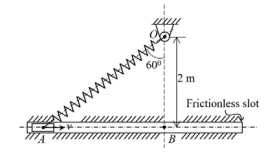
\includegraphics[width=0.6\columnwidth]{q82.png}
    \caption*{}
    \label{fig:q82}
\end{figure}

\hfill{\brak{\text{GATE XE 2022}}}

\item A sphere A of mass $m$ is thrown into the air at 50 m/s along a direction $\tan^{-1}(3/4)$ up from the horizontal. At the topmost point of its trajectory, it has a central (non-oblique) collision with another sphere B which is at rest on top of a vertical pole. Sphere B has a mass of $3m$. Acceleration due to gravity is 10 m/s$^2$. Neglect contact friction and air-resistance. If the coefficient of restitution is 0.3, then the speed (in m/s) of sphere A immediately after the collision is \underline{\hspace{2cm}} (rounded off to one decimal place)

\hfill{\brak{\text{GATE XE 2022}}}

\item The truck shown in the figure is moving on a horizontal road at a speed of 20 m/s. It is carrying a box of mass 1000 kg, which is simply placed on the truck platform. The coefficient of friction between the truck platform and the box is 0.25. Take acceleration due to gravity as 10 m/s$^2$. Assume uniform deceleration during braking, and the coefficients of static and kinetic friction to be the same. The shortest distance in meters in which the truck can be brought to rest without the box slipping is \underline{\hspace{2cm}} (round off to the nearest integer)
\begin{figure}[H]
    \centering
    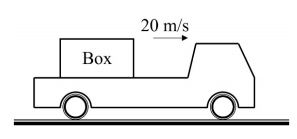
\includegraphics[width=0.6\columnwidth]{q84.png}
    \caption*{}
    \label{fig:q84}
\end{figure}

\hfill{\brak{\text{GATE XE 2022}}}

\item The stepped rod of length 2 m, shown in the figure, is fixed at both ends (A and C). The area of cross-section of portion AB is 200 mm$^2$ and that of portion BC is 100 mm$^2$. Force F is applied at section B such that the section is displaced by 0.1 mm in the direction of the force. Young's modulus of the rod is 200 GPa. The applied force F in N is \underline{\hspace{2cm}} (round off to the nearest integer)
\begin{figure}[H]
    \centering
    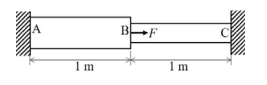
\includegraphics[width=0.6\columnwidth]{q85.png}
    \caption*{}
    \label{fig:q85}
\end{figure}

\hfill{\brak{\text{GATE XE 2022}}}

\item A cantilever beam has a span of 1 m and carries a uniformly distributed load of q = 1250 N/m over a portion as shown. A force F =1000 N acts at a distance L from the fixed end. The distance L is such that the bending moment at the fixed end is zero. The beam has a rectangular cross-section of depth 20 mm and width 24 mm. For this loading, the magnitude of the maximum bending stress in the beam in MPa is \underline{\hspace{2cm}} (round off to the nearest integer)
\begin{figure}[H]
    \centering
    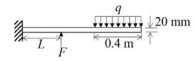
\includegraphics[width=0.5\columnwidth]{q86.png}
    \caption*{}
    \label{fig:q86}
\end{figure}

\hfill{\brak{\text{GATE XE 2022}}}

\item The figure shows two identical mass-less beams AB and CD, each clamped at one of their ends. The left end of beam CD rests on the right end of beam AB such that the ends of the beams are just in contact. The beams are unstressed before the application of load. Assume no friction at the contact. Now, if a uniformly distributed load of 800 N/m is applied on beam CD, the bending moment at the end B of beam AB in N.m is \underline{\hspace{2cm}} (rounded off to the nearest integer)
\begin{figure}[H]
    \centering
    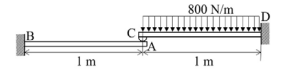
\includegraphics[width=0.6\columnwidth]{q87.png}
    \caption*{}
    \label{fig:q87}
\end{figure}

\hfill{\brak{\text{GATE XE 2022}}}

\item The energy equation for a reversible non-flow process can be expressed as $\delta q = du + p dv$, where q is the heat transfer per unit mass, u is the internal energy per unit mass, p is the pressure, and v is the mass specific volume. This energy equation is not in exact differential form. It can be made exact differential by multiplying with the following integrating factor: (T is the absolute temperature)

\hfill{\brak{\text{GATE XE 2022}}}
\begin{enumerate}
    \item $\frac{1}{p}$
    \item $\frac{1}{v}$
    \item $\frac{1}{T}$
    \item $\frac{1}{uT}$
\end{enumerate}

\item An air standard Diesel cycle consists of four processes: 1-2 (isentropic compression), 2-3 (constant pressure heat addition), 3-4 (isentropic expansion) and 4-1 (constant volume heat rejection). T$_4$ is the temperature (in K) attained at the end of isentropic expansion (3-4) before constant volume heat rejection. The constant volume heat rejection process (4-1) is replaced by a constant pressure heat rejection process (4a-1) such that T$_{4a}$ is the temperature (in K) reached at the end of isentropic expansion (3-4a), and the state point 1 remains the same. Then

\hfill{\brak{\text{GATE XE 2022}}}
\begin{enumerate}
    \item $T_{4a} < T_4$
    \item $T_{4a} > T_4$
    \item $T_{4a} = T_4$
    \item $T_{4a} = 2T_4$
\end{enumerate}

\item Gas in a cylinder-piston device expands from state 1 $(p_1,V_1,T_1)$ to state 2 $(p_2,V_2,T_2)$. The expansion process is polytropic, i.e., $pV^n = \text{constant}, n \neq 1$. Assuming the ideal gas behaviour, the expression for the work done, W by the system is given by

\hfill{\brak{\text{GATE XE 2022}}}
\begin{enumerate}
    \item $W = p_1V_1 \ln{\brak{\frac{T_2}{T_1}}}$
    \item $W = \frac{p_2V_2 - p_1V_1}{1-n}$
    \item $W = p_1V_1 \ln{\brak{\frac{V_1}{V_2}}}$
    \item $W = p_2V_2 \ln{\brak{\frac{p_2}{p_1}}}$
\end{enumerate}

\item The temperature of the working fluid in a real heat engine cycle changes during heat addition and heat rejection processes. The maximum and minimum temperatures of the cycle are T$_{max}$ and T$_{min}$, respectively. If $\eta_C$ is the thermal efficiency of a Carnot engine operating between these temperature limits, then the thermal efficiency, $\eta$ of the real heat engine satisfies the relation

\hfill{\brak{\text{GATE XE 2022}}}
\begin{enumerate}
    \item $\eta > \eta_C$
    \item $\eta < \eta_C$
    \item $\eta = \eta_C$
    \item $\eta = 1 + \eta_C$
\end{enumerate}

\item A 1.2 m$^3$ rigid vessel contains 8 kg of saturated liquid-vapor mixture at 150 kPa. The specific enthalpy of this mixture is \underline{\hspace{2cm}} kJ/kg (round off to 2 decimal places).
At 150 kPa: $v_f = 0.001053 \text{ m}^3/\text{kg}, v_g = 1.1594 \text{ m}^3/\text{kg}$
$h_f = 467.13 \text{ kJ/kg}, h_g = 2693.1 \text{ kJ/kg}$

\hfill{\brak{\text{GATE XE 2022}}}

\item Air in a closed system undergoes a thermodynamic process from an initial temperature of 300 K to the final temperature of 400 K. The specific heat of air at constant volume, $c_v$ varies linearly with the temperature, T (in K) as
$c_v = (0.7 + 0.27 \times 10^{-3} T)$ kJ/(kg K).
Change in the specific internal energy of the air in the system is \underline{\hspace{2cm}} kJ/kg (round off to 2 decimal places).

\hfill{\brak{\text{GATE XE 2022}}}

\item A vertical cylinder-piston device contains a fixed mass of gas in equilibrium. The cross-sectional area of the piston is 0.05 m$^2$. For 150 kPa pressure of the gas in the cylinder, the mass of the piston is \underline{\hspace{2cm}} kg (round off to 2 decimal places).
Assume that the atmospheric pressure is 100 kPa and the acceleration due to gravity is 9.81 m/s$^2$.

\hfill{\brak{\text{GATE XE 2022}}}

\item A steam power plant operates on Rankine cycle. At certain operating condition of the plant, there is a reduction of 20\% net work output (kJ/kg) as compared to 100\% capacity. This reduction will cause the specific steam consumption (kg/kJ) to increase by \underline{\hspace{2cm}} \% (in integer).

\hfill{\brak{\text{GATE XE 2022}}}

\item A Carnot heat pump extracts heat from the environment at 250 K, and supplies 6 kW of heat to a room which is maintained at a constant temperature T$_H$. The heat pump requires a power input of 1 kW for its operation. Then, the temperature of the room T$_H$ is \underline{\hspace{2cm}} K (round off to nearest integer).

\hfill{\brak{\text{GATE XE 2022}}}

\item One of the Maxwell equations is expressed as $\brak{\frac{\partial s}{\partial v}}_T = \brak{\frac{\partial p}{\partial T}}_v$, where s is the entropy per unit mass, v is the mass specific volume, p is the pressure, and T is the temperature. In this expression, s is a continuous function of T and v. The derivatives of s are also continuous. Let $c_v$ be specific heat capacity at constant volume for a gas. Then, $\brak{\frac{\partial c_v}{\partial v}}_T$ can be written as

\hfill{\brak{\text{GATE XE 2022}}}
\begin{enumerate}
    \item $\frac{p}{T}\brak{\frac{\partial^2 p}{\partial T^2}}_v$
    \item $\frac{v}{T}\brak{\frac{\partial^2 p}{\partial v^2}}_T$
    \item $T\brak{\frac{\partial^2 p}{\partial T^2}}_v$
    \item $\frac{1}{T}\brak{\frac{\partial^2 p}{\partial v^2}}_T$
\end{enumerate}

\item The general relation among the properties x, y and z at any state point can be expressed as $\brak{\frac{\partial x}{\partial y}}_z \brak{\frac{\partial y}{\partial z}}_x \brak{\frac{\partial z}{\partial x}}_y = -1$. If p, T and h are continuous functions and $c_p = \brak{\frac{\partial h}{\partial T}}_p$, $\mu$ is the Joule-Thomson coefficient, then $\brak{\frac{\partial h}{\partial p}}_T$ is

\hfill{\brak{\text{GATE XE 2022}}}
\begin{enumerate}
    \item $-\mu c_p$
    \item $c_p T$
    \item $-\frac{c_p}{T}$
    \item $\mu c_p$
\end{enumerate}

\item An air-conditioning system consists of an insulated rigid mixing chamber designed to supply air at 24 $\degree$C to a building. The mixing chamber mixes two air streams: (i) a cold air stream at 10 $\degree$C and mass flow rate $\dot{m}_c$ (kg/s), and (ii) a stream of fresh ambient air at 30 $\degree$C and mass flow rate $\dot{m}_a$ (kg/s). Assume air to be an ideal gas with constant specific heat ($c_p = 1.005$ kJ/(kg K), $\gamma = c_p/c_v = 1.4$). Neglect change in kinetic and potential energies as compared to change in enthalpy. Under the steady state condition, the ratio of the mass flow rates of the two streams ($\dot{m}_c/\dot{m}_a$) is

\hfill{\brak{\text{GATE XE 2022}}}
\begin{enumerate}
    \item $\frac{7}{3}$
    \item $\frac{3}{7}$
    \item $\frac{2}{7}$
    \item $\frac{4}{7}$
\end{enumerate}

\item An ideal gas mixture consists of 80\% N$_2$ and 20\% O$_2$ on mass basis. If the total pressure is 300 kPa, then the partial pressure of N$_2$ (in kPa) is (Molecular weights of N$_2$ = 28 kg/kmol and O$_2$ = 32 kg/kmol)

\hfill{\brak{\text{GATE XE 2022}}}
\begin{enumerate}
    \item 246.15
    \item 230.34
    \item 254.78
    \item 213.54
\end{enumerate}

\item On the basis of the ideal gas equation and van der Waals equation, the temperatures of a gas at pressure 10 MPa and specific volume 0.005 m$^3$/kg would be, respectively (Assume gas constant R = 0.3 kJ/(kg K), a = 0.18 m$^6$ kPa/kg$^2$ and b = 0.0014 m$^3$/kg)

\hfill{\brak{\text{GATE XE 2022}}}
\begin{enumerate}
    \item 166.67 K and 235.89 K
    \item 166.67 K and 206.40 K
    \item 166.67 K and 267.21 K
    \item 166.67 K and 240.90 K
\end{enumerate}

\item An ideal Brayton cycle operates between maximum and minimum temperatures of T$_3$ and T$_1$, respectively. For constant values of T$_3$ and T$_1$, the pressure ratio ($r_p$) for maximum work output is ($\gamma$ is the specific heat ratio of air)

\hfill{\brak{\text{GATE XE 2022}}}
\begin{enumerate}
    \item $\brak{\frac{T_3}{T_1}}^{\frac{\gamma}{\gamma-1}}$
    \item $\brak{\frac{T_3}{T_1}}^{\frac{\gamma}{2(\gamma-1)}}$
    \item $\brak{\frac{T_3}{T_1}}^{\frac{\gamma}{2(\gamma-1)}}$
    \item $\brak{\frac{T_3}{T_1}}^{\frac{2}{\gamma-1}}$
\end{enumerate}

\item An insulated rigid tank of volume 10 m$^3$ contains air initially at 1 MPa and 600 K. A valve connected to the tank is opened, and air is allowed to escape until the temperature inside the tank drops to 400 K. The temperature of the discharged air can be approximated as the average of the initial and final temperatures of the air in the tank. Neglect kinetic and potential energies of the discharged air. Assume that air behaves as an ideal gas with constant specific heat so that internal energy $u = c_vT$ and enthalpy $h = c_pT$. Then, the final pressure of the air in the tank is \underline{\hspace{2cm}} MPa (round off to 2 decimal places). Assume $c_p = 1.005$ kJ/(kg K), $\gamma = c_p/c_v = 1.4$

\hfill{\brak{\text{GATE XE 2022}}}

\item Steam enters a steam turbine at 5 MPa and 600 $\degree$C, and exits as saturated vapor at 50 kPa. Under steady state condition, the turbine loses heat to the surroundings at the rate of 50 kJ per kilogram of steam flowing through the turbine. The ambient temperature is 300 K, and the heat transfer to the surroundings takes place at the outer surface of the turbine at a temperature of 450 K. The irreversibility per unit mass of steam flowing through the turbine is \underline{\hspace{2cm}} kJ/kg (round off to 2 decimal places).
Neglect the change in kinetic and potential energies of the steam, and use the following property values:
Superheated steam at 5 MPa, 600 $\degree$C
$v = 0.07870 \text{ m}^3/\text{kg}, u = 3273.3 \text{ kJ/kg}, h = 3666.9 \text{ kJ/kg}, s = 7.2605 \text{ kJ/(kg K)}$
Saturated vapour at 50 kPa
$v_g = 3.2403 \text{ m}^3/\text{kg}, u_g = 2483.2 \text{ kJ/kg}, h_g = 2645.2 \text{ kJ/kg}, s_g = 7.5931 \text{ kJ/(kg K)}$

\hfill{\brak{\text{GATE XE 2022}}}

\item A heat engine receives heat at 1000 K and rejects heat to the environment at 300 K. The efficiency of the heat engine is half of the efficiency of a Carnot engine operating between the above mentioned temperature limits. The work output from the heat engine is completely used to drive a refrigerator that steadily removes heat from a cold space at 260 K at a rate of 5.2 kW, and rejects the heat to the same environment at 300 K. The COP (coefficient of performance) of the refrigerator is half of the COP of the Carnot refrigerator operating between the same temperature limits as that of the refrigerator. Then, rate of heat supplied to the heat engine is \underline{\hspace{2cm}} kW (round off to 2 decimal places).

\hfill{\brak{\text{GATE XE 2022}}}

\item A room contains air at 25 $\degree$C, 100 kPa and 80\% relative humidity. If the saturation pressure of water vapor at 25 $\degree$C is 3.1698 kPa, then the specific humidity of air is \underline{\hspace{2cm}} kg of water vapor / kg of dry air (round off to 4 decimal places).

\hfill{\brak{\text{GATE XE 2022}}}

\item An insulated rigid container is divided into two parts by a thin partition. One part of the container contains 6 kg of saturated liquid-vapor mixture with a dryness fraction of 0.7 at 0.3 MPa. The other part contains 12 kg of saturated liquid at 0.6 MPa of the same substance. When the partition is removed and the system attains equilibrium, the final specific volume of the mixture is \underline{\hspace{2cm}} m$^3$/kg (round off to 2 decimal places).
Use the following property values:
At 0.3 MPa : $v_f = 0.001073 \text{ m}^3/\text{kg}, v_g = 0.60582 \text{ m}^3/\text{kg}$
At 0.6 MPa : $v_f = 0.001101 \text{ m}^3/\text{kg}, v_g = 0.31560 \text{ m}^3/\text{kg}$

\hfill{\brak{\text{GATE XE 2022}}}

\item During a steady state air-conditioning process, air enters a heating section at 15 $\degree$C with 40\% relative humidity and leaves at 30 $\degree$C. Assuming the heating process takes place at 100 kPa, the relative humidity of the air at exit is \underline{\hspace{2cm}} \% (round off to nearest integer).
Saturation pressures of water vapor at 15 $\degree$C and 30 $\degree$C are 1.7057 kPa and 4.2469 kPa respectively.

\hfill{\brak{\text{GATE XE 2022}}}

\item Steam enters a steam turbine at 10 MPa and 600 $\degree$C with a mass flow rate of 16 kg/s. The steam exits the turbine as saturated vapor at 10 kPa. Under steady state condition, the turbine generates 16.2 MW power. If the ambient temperature is 25 $\degree$C, the rate of entropy generation in the turbine is \underline{\hspace{2cm}} kW/K (round off to 2 decimal places).
Neglect the change in kinetic and potential energies of the steam, and use the following property values:
Superheated steam at 10 MPa, 600 $\degree$C
$v = 0.03837 \text{ m}^3/\text{kg}, u = 3241.68 \text{ kJ/kg}, h = 3625.34 \text{ kJ/kg}, s = 6.9028 \text{ kJ/(kg K)}$
Saturated vapour at 10 kPa
$v_g = 14.67355 \text{ m}^3/\text{kg}, u_g = 2437.89 \text{ kJ/kg}, h_g = 2584.63 \text{ kJ/kg}, s_g = 8.1501 \text{ kJ/(kg K)}$

\hfill{\brak{\text{GATE XE 2022}}}

\item Which of the following is not a caramel flavour producing compound?

\hfill{\brak{\text{GATE XE 2022}}}
\begin{enumerate}
    \item 3-Hydroxy-2-methylpyran-4-one
    \item 2H-4-Hydroxy-5-methylfuran-3-one
    \item 3-Hydroxy-2-acetylfuran
    \item p-Amino benzoicacid
\end{enumerate}

\item Match the size reduction equipment in Column I with the method of operation in Column II.
\begin{table}[h]
    \centering
    \begin{tabular}{|ll|ll|}
    \hline
    \multicolumn{2}{|c|}{\textbf{Column I}} & \multicolumn{2}{c|}{\textbf{Column II}} \\
    \hline
    P. & Hammer mill & 1. & Compression \\
    Q. & Burr mill & 2. & Impact \\
    R. & Crushing rolls & 3. & Cutting \\
    S. & Rotary knife & 4. & Attrition \\
    \hline
    \end{tabular}
    \caption*{}
    \label{tab:q144}
\end{table}

\hfill{\brak{\text{GATE XE 2022}}}
\begin{enumerate}
    \item P-2, Q-4, R-1, S-3
    \item P-3, Q-1, R-2, S-4
    \item P-4, Q-1, R-2, S-3
    \item P-3, Q-4, R-2, S-1
\end{enumerate}

\item Most commonly used refrigerant in direct immersion freezing of food is

\hfill{\brak{\text{GATE XE 2022}}}
\begin{enumerate}
    \item Monochlorodifluoromethane
    \item Dichlorodifluoromethane
    \item Liquid nitrogen
    \item Freon
\end{enumerate}

\item Which among the following are $\omega$-6 poly unsaturated essential fatty acids?

\hfill{\brak{\text{GATE XE 2022}}}
\begin{enumerate}
    \item 18:2 Linoleic acid
    \item 18:3 $\alpha$-Linolenic acid
    \item 18:3 $\gamma$-Linolenic acid
    \item 20:4 Arachidonic acid
\end{enumerate}

\item Which among the following statements are true with respect to protein denaturation?

\hfill{\brak{\text{GATE XE 2022}}}
\begin{enumerate}
    \item There may be an increase in $\alpha$-helix and $\beta$-sheet structure
    \item It is an irreversible process
    \item When fully denatured, globular proteins resemble a random coil
    \item The peptide bonds are broken
\end{enumerate}

\item Identify the correct pair(s) of milling equipment and the grain for which it is used.

\hfill{\brak{\text{GATE XE 2022}}}
\begin{enumerate}
    \item Mist polisher-Rice
    \item Break roll-Wheat
    \item Rubber roll-Pigeon pea
    \item Beall degermer-Maize
\end{enumerate}

\item Which among the following expression(s) is/are correct?

\hfill{\brak{\text{GATE XE 2022}}}
\begin{enumerate}
    \item Reynolds number = $\frac{\text{Density} \times \text{Velocity} \times \text{Characteristic dimension}}{\text{Viscosity}}$
    \item Nusselt number = $\frac{\text{Convective heat transfer coefficient} \times \text{Characteristic dimension}}{\text{Thermal conductivity of solid}}$
    \item Schmidt number = $\frac{\text{Kinematic viscosity of fluid}}{\text{diffusivity}}$
    \item Biot number = $\frac{\text{Convective heat transfer coefficient} \times \text{Characteristic dimension}}{\text{Thermal conductivity of fluid}}$
\end{enumerate}

\item In sieve analysis of coffee powder, the particle size distribution is given below
\begin{table}[h]
    \centering
    \begin{tabular}{|c|c|}
    \hline
    Number of particles & Mean particle size ($\mu$m) \\
    \hline
    5 & 40 \\
    8 & 30 \\
    50 & 20 \\
    90 & 17.5 \\
    148 & 12.5 \\
    10 & 10 \\
    \hline
    \end{tabular}
    \caption*{}
    \label{tab:q150}
\end{table}
The Sauter mean diameter (in $\mu$m) of the coffee powder is \underline{\hspace{2cm}}
(round off to one decimal place).

\hfill{\brak{\text{GATE XE 2022}}}

\item In a dairy processing plant, milk enters a 30 m long and 2 cm diameter tube at 60 $\degree$C and leaves at 57 $\degree$C. The total heat loss over the tube length is 381.15 W. The specific heat capacity, density, and viscosity of milk are 3.85 kJ kg$^{-1}$ K$^{-1}$, 1020 kg m$^{-3}$, and 1.20 cP, respectively. The Reynolds number for the flow is \underline{\hspace{2cm}} (round off to the nearest integer). Given: $\pi = 3.14$

\hfill{\brak{\text{GATE XE 2022}}}

\item Apple juice flows through a steel pipe having thermal conductivity of 50 W m$^{-1}$ K$^{-1}$. The outer surface of pipe is exposed to ambient environment. The inside diameter and thickness of the pipe are 3 cm and 1.5 cm, respectively. The overall heat transfer coefficient based on inside area is 25 W m$^{-2}$ K$^{-1}$. If the internal convective heat transfer coefficient is 30 W m$^{-2}$ K$^{-1}$, the external convective heat transfer coefficient (in W m$^{-2}$ K$^{-1}$) will be \underline{\hspace{2cm}} (round off to two decimal places).

\hfill{\brak{\text{GATE XE 2022}}}

\item The dry bulb temperature and relative humidity of air inside a storage chamber are 37 $\degree$C and 50\%, respectively. The saturation pressure of water vapour at 37 $\degree$C and barometric pressure are 6.28 kPa and 101.32 kPa, respectively. The humidity ratio of air inside the chamber is \underline{\hspace{2cm}} kg water (kg dry air)$^{-1}$ (round off to three decimal places). Given: Molecular weight of water vapour and dry air are 18.02 g mol$^{-1}$ and 28.97 g mol$^{-1}$, respectively.

\hfill{\brak{\text{GATE XE 2022}}}

\item The figure shows a schematic of vertical profiles of concentrations of two gases P and Q in the atmosphere near a coastal station. The correct pair representing P and Q, respectively, is
\begin{figure}[H]
    \centering
    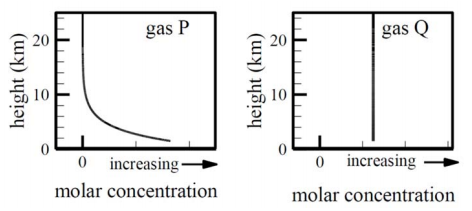
\includegraphics[width=0.7\columnwidth]{q154.png}
    \caption*{}
    \label{fig:q154}
\end{figure}

\hfill{\brak{\text{GATE XE 2022}}}
\begin{enumerate}
    \item water vapor and CO$_2$
    \item O$_3$ and water vapor
    \item CO$_2$ and O$_3$
    \item N$_2$ and O$_2$
\end{enumerate}

\item A form of momentum equation for an incompressible fluid is
$\rho \frac{DV}{Dt} = -\nabla p + \mu \nabla^2 V + B$
(i) \hspace{1cm} (ii) \hspace{1cm} (iii) \hspace{1cm} (iv)
where $\rho$ is density, V is velocity, t is time, p is pressure, $\mu$ is viscosity and B represents body force per unit volume. The dimension of term (iii) is (M, L and T stand for mass, length and time, respectively).

\hfill{\brak{\text{GATE XE 2022}}}
\begin{enumerate}
    \item [L]$^1$ [T]$^{-2}$
    \item [M]$^1$ [L]$^{-2}$ [T]$^{-2}$
    \item [M]$^1$ [L]$^1$ [T]$^{-2}$
    \item [M]$^1$ [L]$^1$ [T]$^{-1}$
\end{enumerate}

\item Tropical cyclones usually do not form close to the Equator primarily because

\hfill{\brak{\text{GATE XE 2022}}}
\begin{enumerate}
    \item sea surface temperature at the Equator is too cold.
    \item beta effect dissipates clouds.
    \item Coriolis force is too weak.
    \item vertical shear of the zonal wind is weak.
\end{enumerate}

\item Which one of the following statements regarding equatorial under current (EUC) in the Pacific Ocean is correct?

\hfill{\brak{\text{GATE XE 2022}}}
\begin{enumerate}
    \item EUC flows from west to east.
    \item EUC flows from east to west.
    \item EUC flows from north to south.
    \item EUC flows from south to north.
\end{enumerate}

\item Which one of the following statements is correct regarding the dominant energy balance in the troposphere in a tropical convergence zone?

\hfill{\brak{\text{GATE XE 2022}}}
\begin{enumerate}
    \item Shortwave heating balances longwave radiative cooling.
    \item Compressional heating balances radiative cooling.
    \item Radiative cooling balances heating due to viscous dissipation of kinetic energy.
    \item Condensational heating balances adiabatic cooling.
\end{enumerate}

\item Which one of the following processes is primarily responsible for the poleward transport of energy in the midlatitude troposphere?

\hfill{\brak{\text{GATE XE 2022}}}
\begin{enumerate}
    \item atmospheric tides
    \item baroclinic waves
    \item gravity waves
    \item turbulence in the boundary layer
\end{enumerate}

\item Which of the following feature(s) characterize the seasonal mean flow in the upper troposphere near 200 hPa level over the Tibetan Plateau during the boreal summer?

\hfill{\brak{\text{GATE XE 2022}}}
\begin{enumerate}
    \item cyclonic
    \item anticyclonic
    \item irrotational
    \item divergent
\end{enumerate}

\item The Rossby number of a synoptic system with a length scale of 1000 km, characteristic velocity scale of 10 m s$^{-1}$ at a latitude where the Coriolis parameter equals 10$^{-4}$ s$^{-1}$, is \underline{\hspace{2cm}}. (Round off to two decimal places)

\hfill{\brak{\text{GATE XE 2022}}}

\item The ratio of scattering efficiency of red light of wavelength 0.65 $\mu$m to blue light of wavelength 0.45 $\mu$m by air molecules in the atmosphere is \underline{\hspace{2cm}}. (Round off to two decimal places)

\hfill{\brak{\text{GATE XE 2022}}}

\item An unsaturated moist air parcel undergoes adiabatic ascent in atmosphere without mixing with surrounding air. Air is so clean that there is no possibility for heterogeneous nucleation. Which one of the following plots depicts the vertical variation of water vapor pressure (shown as continuous line) and saturation water vapor pressure (shown as dotted/dashed line) of the parcel?
\begin{figure}[H]
    \centering
    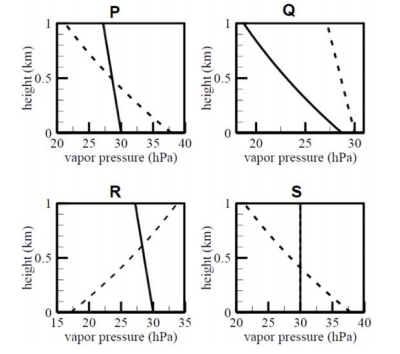
\includegraphics[width=0.8\columnwidth]{q163.png}
    \caption*{}
    \label{fig:q163}
\end{figure}

\hfill{\brak{\text{GATE XE 2022}}}
\begin{enumerate}
    \item P
    \item Q
    \item R
    \item S
\end{enumerate}

\item A fluid is in solid body rotation in a cylindrical container of radius R rotating with an angular velocity $\Omega = (0, 0, \Omega)$. The circulation per unit area around a circular loop in the horizontal plane of radius r (r $<$ R), whose center coincides with the axis of rotation is

\hfill{\brak{\text{GATE XE 2022}}}
\begin{enumerate}
    \item 2 $\Omega$
    \item $\Omega^2$
    \item $\Omega$/2
    \item $\Omega$/4
\end{enumerate}

\item Consider a layer of atmosphere where temperature increases with height. If the concentration of a vertically well-mixed greenhouse gas suddenly increases in this layer, then an immediate consequence is that

\hfill{\brak{\text{GATE XE 2022}}}
\begin{enumerate}
    \item infrared radiation leaving the top of the layer decreases.
    \item infrared radiation leaving the top of the layer increases.
    \item infrared radiation leaving the top of the layer remains unchanged.
    \item the layer becomes optically thinner to infrared radiation.
\end{enumerate}

\item Consider an atmosphere where the mole fractions of N$_2$, Ar and CO$_2$ are $7.81 \times 10^{-1}$, $9.34 \times 10^{-3}$ and $4.05 \times 10^{-4}$, respectively. This atmosphere exchanges gases with sea water below having temperature and salinity of 20 $\degree$C and 35 psu, respectively. In the absence of biological and chemical activity, relative concentrations of dissolved gases in the surface sea water at equilibrium are ordered as

\hfill{\brak{\text{GATE XE 2022}}}
\begin{enumerate}
    \item [N$_2$] $>$ [Ar] $>$ [CO$_2$]
    \item [CO$_2$] $>$ [N$_2$] $>$ [Ar]
    \item [N$_2$] $>$ [CO$_2$] $>$ [Ar]
    \item [Ar] $>$ [CO$_2$] $>$ [N$_2$]
\end{enumerate}

\item Gravitational forces exerted by the Sun and the Moon are mainly responsible for ocean tides. Which of the following statement(s) regarding ocean tides is/are correct?

\hfill{\brak{\text{GATE XE 2022}}}
\begin{enumerate}
    \item Tidal amplitude corresponding to diurnal period is larger than that of the semi-diurnal period.
    \item Diurnal time period of lunar forced tides is longer than that of the solar forced tides.
    \item Tidal amplitudes are larger during a solar eclipse compared to that during a lunar eclipse.
    \item Tides are absent during equinoxes.
\end{enumerate}

\item Which of the following statement(s) is/are true about northern hemisphere tropical cyclones?

\hfill{\brak{\text{GATE XE 2022}}}
\begin{enumerate}
    \item They have a warm core.
    \item Their low-level flow is cyclonic.
    \item Strong wind shear in the vertical is required for their intensification.
    \item They are characterized by upper-level divergence.
\end{enumerate}

\item In gradient wind balance, which of the following statement(s) is/are true for flow around a region of low pressure in the northern hemisphere?

\hfill{\brak{\text{GATE XE 2022}}}
\begin{enumerate}
    \item The flow is clockwise.
    \item The flow is anti-clockwise.
    \item The wind speed is faster than the geostrophic wind.
    \item The wind speed is slower than the geostrophic wind.
\end{enumerate}

\item Which of the following statement(s) is/are true regarding biogeochemical cycle in the ocean?

\hfill{\brak{\text{GATE XE 2022}}}
\begin{enumerate}
    \item Shutdown of the biological pump in the ocean would have resulted in higher CO$_2$ concentration in the atmosphere compared to present-day.
    \item If atmospheric CO$_2$ concentration increases, solubility pump would lead to a decrease in dissolved inorganic carbon in the ocean.
    \item All carbon sequestered by marine photosynthesis settles down on the ocean floor as organic matter.
    \item Calcification (the process of making shells and skeletons) by marine organisms in the surface ocean layer would lead to an increase in the surface ocean CO$_2$.
\end{enumerate}

\item Consider the atmosphere to be a heat engine, which converts absorbed radiation to kinetic energy of winds. Let the global mean radiation absorbed be 200 Wm$^{-2}$. In steady-state, if the global mean kinetic energy dissipation is 10 Wm$^{-2}$, then the efficiency of the atmospheric heat engine is \underline{\hspace{2cm}} \%. (Round off to one decimal place)

\hfill{\brak{\text{GATE XE 2022}}}

\item A drifter on the surface of the ocean performs inertial oscillation. The speed of the drifter is 2 m s$^{-1}$ and the Coriolis parameter at the latitude is $2 \times 10^{-4}$ s$^{-1}$. The radius of the inertial oscillation is \underline{\hspace{2cm}} km. (Round off to the nearest integer)

\hfill{\brak{\text{GATE XE 2022}}}

\item Consider a tornado in cyclostrophic balance. The tangential wind speed at a radial distance of 500 m from the center of the tornado is \underline{\hspace{2cm}} m s$^{-1}$, if the pressure gradient at that location in the radial direction is 5 N m$^{-3}$. Assume the density of air to be 1 kg m$^{-3}$. (Round off to the nearest integer)

\hfill{\brak{\text{GATE XE 2022}}}

\item Consider two weather stations A and B having the same altitude. Station B is 5 km north of Station A and is always 2 K warmer than Station A. A steady northerly wind blows at 1 m s$^{-1}$. The change in temperature at Station A in 2 hours is \underline{\hspace{2cm}} K. (Round off to one decimal place)

\hfill{\brak{\text{GATE XE 2022}}}

\item Assume the Earth is in radiative equilibrium with effective radiative temperature of 255 K. If the planetary albedo increases by 0.05, then the effective radiative temperature of the planet will be \underline{\hspace{2cm}} K. (Round off to the nearest integer)
Given:
Solar constant = 1370 Wm$^{-2}$
Stefan Boltzmann constant = $5.67 \times 10^{-8}$ Wm$^{-2}$ K$^{-4}$

\hfill{\brak{\text{GATE XE 2022}}}

\end{enumerate}

\end{document}